\documentclass{beamer}

\usepackage[utf8x]{inputenc}
\usepackage{graphicx}
\usepackage{amsthm,amssymb,amsbsy,amsmath,amsfonts,amssymb,amscd}
\usepackage{tikz}
\usepackage{dsfont}
\usepackage{array}
\newcolumntype{N}{@{}m{2pt}@{}}
\input{style.tex}

\title[Introduction to Gaussian Process Surrogates Models]{ \small MDIS Fall School 2017\\ \vspace{3mm} \Large Introduction to Gaussian Process Surrogate models}
\institute{Nicolas Durrande, PROWLER.io (nicolas@prowler.io) \\ Rodolphe Le Riche, CNRS LIMOS -- Mines St-\'Etienne (leriche@emse.fr)}
\author[MDIS 2017]{Clermont-Ferrand, Besse-en-Chandesse, 16th of October 2017}
\date{\texttt{http://github.com/NicolasDurrande/intro\_to\_GPs\_with\_R}}

\DeclareMathOperator*{\Var}{var}
\DeclareMathOperator*{\E}{E}
\DeclareMathOperator*{\Cov}{cov}
\newcommand\PR[1]{\mathrm{P}\left(#1 \right)}
\newcommand\PS[1]{{\langle #1 \rangle}_\mathcal{H}}
\newcommand\PSi[2]{{ \left \langle #1 \right \rangle}_{\! #2}}
\newcommand\N[1]{{|| #1 ||}_\mathcal{H}}
\newcommand\Ni[2]{{|| #1 ||}_{\! #2}}
\newcommand\dx{\, \mathrm{d}}
\newcommand\textequal{\rule[.4ex]{4pt}{0.4pt}\llap{\rule[.7ex]{4pt}{0.4pt}}}
\newcommand{\argmin}{\operatornamewithlimits{argmin}}
\makeatletter
\newcommand{\shorteq}{%
    \settowidth{\@tempdima}{a}% Width of hyphen
      \resizebox{\@tempdima}{\height}{=}%
      }
\makeatother

\definecolor{Orange}{rgb}{0.8, 0.147, 0.0}
\definecolor{MonBleu}{rgb}{0.212, 0.392, 0.545}
%%%%%%%%%%%%%%%%%%%%%%%%%%%%%%%%%%%%%%%%%%%%%%%%%%%%%%
%%%%%%%%%%%%%%%%%%%%%%%%%%%%%%%%%%%%%%%%%%%%%%%%%%%%%%
%%%%%%%%%%%%%%%%%%%%%%%%%%%%%%%%%%%%%%%%%%%%%%%%%%%%%%
\begin{document}

%%%%%%%%%%%%%%%%%%%%%%%%%%%%%%%%%%%%%%%%%%%%%%%%%%%%%%
\begin{frame}
  \titlepage
\end{frame}

%%%%%%%%%%%%%%%%%%%%%%%%%%%%%%%%%%%%%%%%%%%%%%%%%%%%%%
%%%%%%%%%%%%%%%%%%%%%%%%%%%%%%%%%%%%%%%%%%%%%%%%%%%%%%
\section[Statistical Models]{Statistical models in engineering?}
\subsection{}
%%%%%%%%%%%%%%%%%%%%%%%%%%%%%%%%%%%%%%%%%%%%%%%%%%%%%%
\begin{frame}{}
There is a wide variety of situations where getting data about a system performance can be extremely expensive.
\begin{itemize}
	\item real world experiments
	\item destructive tests
	\item prototyping
	\item numerical experiments
\end{itemize}
\end{frame}

%%%%%%%%%%%%%%%%%%%%%%%%%%%%%%%%%%%%%%%%%%%%%%%%%%%%%%
\begin{frame}{}
\begin{exampleblock}{Example: real world experiments}
\begin{center}
\includegraphics[height=5cm]{1_stat_models/figures/drilling}
\end{center}
\end{exampleblock}
\end{frame}

%%%%%%%%%%%%%%%%%%%%%%%%%%%%%%%%%%%%%%%%%%%%%%%%%%%%%%
\begin{frame}{}
\begin{exampleblock}{Example: Destructive tests}
\begin{center}
\includegraphics[height=5cm]{1_stat_models/figures/crash-test}
\end{center}
\end{exampleblock}
\end{frame}

%%%%%%%%%%%%%%%%%%%%%%%%%%%%%%%%%%%%%%%%%%%%%%%%%%%%%%
\begin{frame}{}
\begin{exampleblock}{Example: Prototyping of a boat shape}
\begin{center}
\includegraphics[height=3.5cm]{1_stat_models/figures/carene} \qquad \includegraphics[height=3.5cm]{1_stat_models/figures/carene2}
\end{center}
Knowing the drag for a given design requires costly experiments
\end{exampleblock}
\end{frame}

%%%%%%%%%%%%%%%%%%%%%%%%%%%%%%%%%%%%%%%%%%%%%%%%%%%%%%
\begin{frame}{}
\begin{exampleblock}{Example: Numerical experiments}
\begin{center}
\includegraphics[height=2.8cm]{1_stat_models/figures/waterflow} \qquad \includegraphics[height=4.2cm]{1_stat_models/figures/crash/image15}
\end{center}
Numerical experiments are less expensive but can be very time consuming!
\end{exampleblock}
\end{frame}

%%%%%%%%%%%%%%%%%%%%%%%%%%%%%%%%%%%%%%%%%%%%%%%%%%%%%%
\begin{frame}{}
In all these cases, the variable of interest can be seen as a function of the input parameters
$$ y = f(x). $$
where $f$ is a \textbf{costly to evaluate function}. \\
\vspace{5mm}
In the following, we will assume that
\begin{itemize}
	\item $x \in \mathds{R}^d$: There are many input parameters
	\item $y \in \mathds{R}$: The output is a scalar.
\end{itemize}
\end{frame}

%%%%%%%%%%%%%%%%%%%%%%%%%%%%%%%%%%%%%%%%%%%%%%%%%%%%%%
\begin{frame}{}
The fact that $f$ is \textbf{costly to evaluate} changes a lot of things...\\
\vspace{5mm}
\structure{1. Representing the function is not possible...}\\
\vspace{5mm}
\begin{center}
\includegraphics[height=3.2cm]{1_stat_models/figures/ink_f} \includegraphics[height=3.2cm]{1_stat_models/figures/Rightarrow} \includegraphics[height=3.2cm]{1_stat_models/figures/ink_fX}
\end{center}
\end{frame}

%%%%%%%%%%%%%%%%%%%%%%%%%%%%%%%%%%%%%%%%%%%%%%%%%%%%%%
\begin{frame}{}
The fact that $f$ is \textbf{costly to evaluate} changes a lot of things...\\
\vspace{5mm}
\structure{2. Computing integrals is not possible...}\\
\vspace{5mm}
\begin{center}
\includegraphics[height=4.5cm]{1_stat_models/figures/ink_fX}
\end{center}
What is the mean value of $f$?
\end{frame}

%%%%%%%%%%%%%%%%%%%%%%%%%%%%%%%%%%%%%%%%%%%%%%%%%%%%%%
\begin{frame}{}
The fact that $f$ is \textbf{costly to evaluate} changes a lot of things...\\
\vspace{5mm}
\structure{3. Uncertainty propagation is not possible...}\\
\vspace{5mm}
\begin{center}
\includegraphics[height=3.2cm]{1_stat_models/figures/ink_unprogf} \includegraphics[height=3.2cm]{1_stat_models/figures/Rightarrow} \includegraphics[height=3.2cm]{1_stat_models/figures/ink_unprogfX}
\end{center}
\end{frame}

%%%%%%%%%%%%%%%%%%%%%%%%%%%%%%%%%%%%%%%%%%%%%%%%%%%%%%
\begin{frame}{}
The fact that $f$ is \textbf{costly to evaluate} changes a lot of things...\\
\vspace{5mm}
\structure{4. Sensitivity analysis is not possible...}\\
\vspace{5mm}
\begin{center}
\includegraphics[height=4.5cm]{1_stat_models/figures/ink_as}
\end{center}
\end{frame}

%%%%%%%%%%%%%%%%%%%%%%%%%%%%%%%%%%%%%%%%%%%%%%%%%%%%%%
\begin{frame}{}
The fact that $f$ is \textbf{costly to evaluate} changes a lot of things...\\
\vspace{5mm}
\structure{5. Optimisation is also tricky...}\\
\vspace{5mm}
\begin{center}
\includegraphics[height=4.5cm]{1_stat_models/figures/ink_fX}
\end{center}
\end{frame}

%%%%%%%%%%%%%%%%%%%%%%%%%%%%%%%%%%%%%%%%%%%%%%%%%%%%%%
\begin{frame}{}
The principle of statistical modelling is to use the data to build a mathematical approximation of the function.
\begin{center}
\includegraphics[height=4.5cm]{1_stat_models/figures/ink_m}
\end{center}
The model can then be used to answer all previous questions
\end{frame}

%%%%%%%%%%%%%%%%%%%%%%%%%%%%%%%%%%%%%%%%%%%%%%%%%%%%%%
\begin{frame}{}
Of course, there is a difference between $f$ and $m$...
\begin{center}
\includegraphics[height=5cm]{1_stat_models/figures/ink_mf}
\end{center}
\end{frame}

%%%%%%%%%%%%%%%%%%%%%%%%%%%%%%%%%%%%%%%%%%%%%%%%%%%%%%
\begin{frame}{}
Why \textbf{statistical models}? \\We want to be able to quantify the model error:
\begin{center}
\includegraphics[height=5cm]{1_stat_models/figures/ink_mconfint}
\end{center}
The confidence intervals can be used to obtain a \textbf{measure of uncertainty on the value of interest}.
\end{frame}

%%%%%%%%%%%%%%%%%%%%%%%%%%%%%%%%%%%%%%%%%%%%%%%%%%%%%%
\begin{frame}{}
In the sequel, we will use the following notations :
\begin{itemize}
	\item The set of observation points will be represented by a $n \times d$ matrix $X=(X_1, ..., X_n)^t$
	\item The vector of observations will be denoted by $F$ : $F_i=f(X_i)$ (or $F=f(X)$).
\end{itemize}
There are many surrogate methods available on the market
\begin{itemize}
	\item Linear regression
	\item Smoothing splines
	\item Gaussian process regression
	\item Neural Networks
    \item ...
\end{itemize}
In this course we will focus on \textbf{Gaussian Process Regression}.
\end{frame}

%%%%%%%%%%%%%%%%%%%%%%%%%%%%%%%%%%%%%%%%%%%%%%%%%%%%%%
%%%%%%%%%%%%%%%%%%%%%%%%%%%%%%%%%%%%%%%%%%%%%%%%%%%%%%
\section[Gaussian Process regression]{Gaussian Process Regression}
\subsection{}
%%%%%%%%%%%%%%%%%%%%%%%%%%%%%%%%%%%%%%%%%%%%%%%%%%%%%%
\begin{frame}{}
\vspace{0.75cm}
\structure{This section is be organised in 3 subsections:}
\vspace{0.5cm}
\begin{enumerate}
    \item Reminders on Multivariate normal distribution
    \item Gaussian processes
    \item Gaussian process regression
\end{enumerate}
\end{frame}

%%%%%%%%%%%%%%%%%%%%%%%%%%%%%%%%%%%%%%%%%%%%%%%%%%%%%%%%%%%%
%\subsection{Multivariate normal distribution}

%%%%%%%%%%%%%%%%%%%%%%%%%%%%%%%%%%%%%%%%%%%%%%%%%%%%%%
\begin{frame}{1. Multivariate normal distribution}
The usual one dimensional normal distribution $\mathcal{N}(\mu,\sigma^2)$ has the following pdf:
\begin{equation*}
f(x) = \frac{1}{\sigma \sqrt{2 \pi}} \exp \left(-\frac{(x-\mu)^2}{2 \sigma^2} \right) \text{ for } x \in \mathds{R}
\end{equation*}
It can be generalised to vectors:
\begin{definition}
	We say that a vector $Y=(Y_1, \dots, Y_n)$ follows a multivariate normal distribution if any linear combination of $Y$ follows a normal distribution:
	\begin{equation*}
		\forall \alpha \in \mathds{R}^n,\ \alpha^t Y \sim \mathcal{N}(m,s^2)
	\end{equation*}
\end{definition}
\end{frame}

%%%%%%%%%%%%%%%%%%%%%%%%%%%%%%%%%%%%%%%%%%%%%%%%%%%%%%
\begin{frame}{}
The distribution of a Gaussian vector is characterised by
\begin{itemize}
 	\item a mean vector $\mu = (\mu_1, \dots, \mu_d)$
 	\item a $d \times d$ covariance matrix $\Sigma$ : $\Sigma_{i,j}=\Cov(Y_i, Y_j)$
\end{itemize}
\vspace{5mm}
\structure{Property:}\\
A covariance matrix is
\begin{itemize}
	\item \textbf{symmetric} $K_{i,j}=K_{j,i}$
	\item \textbf{positive semi-definite} $\forall \alpha \in \mathds{R}^d, \alpha^t K \alpha \geq 0$.
\end{itemize}
\end{frame}

%%%%%%%%%%%%%%%%%%%%%%%%%%%%%%%%%%%%%%%%%%%%%%%%%%%%%%
\begin{frame}{}
The density of a multivariate Gaussian is:
\begin{equation*}
f_Y(x) = \frac{1}{\displaystyle (2 \pi)^{d/2} |\Sigma|^{1/2}} \exp \left(-\frac12 (x-\mu)^t \Sigma^{-1} (x-\mu)  \right).
\end{equation*}
\begin{center}
 \includegraphics[height=4.7cm]{1_stat_models/figures/R/MVN_dens1} \qquad \includegraphics[height=5cm]{1_stat_models/figures/R/MVN_dens2}
\end{center}
\end{frame}


%%%%%%%%%%%%%%%%%%%%%%%%%%%%%%%%%%%%%%%%%%%%%%%%%%%%%%
\begin{frame}{}
\begin{example}
\begin{center}
 \includegraphics[height=5cm]{1_stat_models/figures/R/MVN_gaussvec2} \quad \includegraphics[height=5cm]{1_stat_models/figures/R/MVN_gaussvec1}
\end{center}
\end{example}
\end{frame}

%%%%%%%%%%%%%%%%%%%%%%%%%%%%%%%%%%%%%%%%%%%%%%%%%%%%%%
\begin{frame}{}
\begin{exampleblock}{Counter example}
\begin{center}
 \includegraphics[height=5cm]{1_stat_models/figures/R/MVN_gaussvec3}
\end{center}
$Y_1$ and $Y_2$ are normally distributed but \textbf{the couple $(Y_1,Y_2)$ is not}.
\end{exampleblock}
\end{frame}


%%%%%%%%%%%%%%%%%%%%%%%%%%%%%%%%%%%%%%%%%%%%%%%%%%%%%%
\begin{frame}{}
\begin{block}{Conditional distribution}
Let $(Y,Z)$ be a Gaussian vector ($Y$ and $Z$ may both be vectors) with mean $(\mu_Y,\mu_Z)^t$ and covariance matrix
\begin{equation*}
\begin{pmatrix}
	\Cov(Y,Y) & \Cov(Y,Z)\\
	\Cov(Z,Y) & \Cov(Z,Z)\\
\end{pmatrix}.
\end{equation*}
The conditional distribution of $Y$ knowing $Z$ is still multivariate normal $Y|Z \sim \mathcal{N}(\mu_{cond},\Sigma_{cond})$ with
\begin{equation*}
\begin{split}
	\mu_{cond} &= \E [Y|Z] = \mu_Y + \Cov(Y,Z) \Cov(Z,Z)^{-1} (Z-\mu_Z)\\
	\Sigma_{cond} &= \Cov [Y,Y|Z] = \Cov(Y,Y) - \Cov(Y,Z) \Cov(Z,Z)^{-1} \Cov(Z,Y)
\end{split}
\end{equation*}
\end{block}
\end{frame}

%%%%%%%%%%%%%%%%%%%%%%%%%%%%%%%%%%%%%%%%%%%%%%%%%%%%%%
\begin{frame}{}
\begin{exampleblock}{Example 1}
2D multivariate Gaussian conditional distribution:\\
\begin{center}
\includegraphics[height=6cm]{1_stat_models/figures/ch1_condpdf1}
\end{center}
\end{exampleblock}
\end{frame}

%%%%%%%%%%%%%%%%%%%%%%%%%%%%%%%%%%%%%%%%%%%%%%%%%%%%%%
\begin{frame}{}
\begin{exampleblock}{Example 2}
3D multivariate Gaussian conditional distribution:\\
\begin{center}
\includegraphics[height=6cm]{1_stat_models/figures/ch1_condpdf2}
\end{center}
\end{exampleblock}
\end{frame}


%%%%%%%%%%%%%%%%%%%%%%%%%%%%%%%%%%%%%%%%%%%%%%%%%%%%%%
\begin{frame}{}
\begin{exampleblock}{Exercise}
	Starting from the density function, prove the previous property using the Schur bloc inverse:
\begin{equation*}
\begin{pmatrix}
	\Sigma_{1,1} & \Sigma_{1,2}\\
	\Sigma_{2,1} & \Sigma_{2,2}\\
\end{pmatrix}^{-1} =
\begin{pmatrix}
	A & B\\
	B^t & C\\
\end{pmatrix}
\end{equation*}
\begin{equation*}
\begin{split}
 \text{where: \quad} A &= (\Sigma_{1,1} - \Sigma_{1,2} \Sigma_{2,2}^{-1} \Sigma_{2,1})^{-1}\\
 B &= -(\Sigma_{1,1} - \Sigma_{1,2} \Sigma_{2,2}^{-1} \Sigma_{2,1})^{-1}\Sigma_{1,2}\Sigma_{2,2}^{-1}\\
 C &= \Sigma_{2,2}^{-1} + \Sigma_{2,2}^{-1} \Sigma_{2,1} (\Sigma_{1,1} -\Sigma_{1,2} \Sigma_{2,2}^{-1} \Sigma_{2,1})^{-1}\Sigma_{1,2}\Sigma_{2,2}^{-1}
\end{split}
\end{equation*}
\end{exampleblock}
\end{frame}

%%%%%%%%%%%%%%%%%%%%%%%%%%%%%%%%%%%%%%%%%%%%%%%%%%%%%%%%%%%%
%\subsection{Gaussian processes}

%%%%%%%%%%%%%%%%%%%%%%%%%%%%%%%%%%%%%%%%%%%%%%%%%%%%%%
\begin{frame}{2. Gaussian processes}
The multivariate Gaussian distribution can be generalised to random processes:
\begin{definition}
A random process $Z$ over $D \subset \mathds{R}^d$ is said to be Gaussian if
\begin{equation*}
\forall n \in \mathds{N}, \forall x_i \in D, (Z(x_1),\dots,Z(x_n)) \text{  is a Gaussian vector}.
\end{equation*}
\end{definition}
The distribution of a GP is fully characterised by:
\begin{itemize}
	\item its mean function $m$ defined over $D$
	\item its covariance function (or kernel) $k$ defined over $D \times D$: $k(x,y) = \Cov(Z(x),Z(y))$
\end{itemize}
We will use the notation $Z \sim \mathcal{N}(m(.),k(.,.))$.
\end{frame}

%%%%%%%%%%%%%%%%%%%%%%%%%%%%%%%%%%%%%%%%%%%%%%%%%%%%%%
\begin{frame}{}
A kernel satisfies the following properties:
\begin{itemize}
	\item It is symmetric: $k(x,y) = k(y,x)$
	\item It is positive semi-definite (psd):
\end{itemize}
\begin{equation*}
	\forall n \in \mathds{N}, \forall x_i \in D, \forall \alpha \in \mathds{R}^n,\  \sum_{i=1}^n \sum_{j=1}^n \alpha_i \alpha_j k(x_i,x_j) \geq 0
\end{equation*}
\vspace{5mm} \\
Furthermore any symmetric psd function can be seen as the covariance of a Gaussian process. This equivalence is known as the Loeve theorem.
\end{frame}

%%%%%%%%%%%%%%%%%%%%%%%%%%%%%%%%%%%%%%%%%%%%%%%%%%%%%%
\begin{frame}{}
Proving that a function is psd is often intractable. However there are a lot of functions that have already been proven to be psd:\\
\vspace{2mm}
\footnotesize
\begin{tabular}{rlN}
		constant & $ \displaystyle k(x,y) = 1 $ &\\[4mm]
		white noise & $ \displaystyle k(x,y) = \delta_{x,y} $ &\\[4mm]
		Brownian & $ \displaystyle k(x,y) =  \min (x,y) $ &\\[4mm]
		exponential & $\displaystyle k(x,y) = \exp \left(- |x-y| \right)$ &\\[4mm]
		Matern 3/2 & $\displaystyle k(x,y) = \left(1 + |x-y| \right) \exp \left(- |x-y| \right)$ &\\[4mm]
		Matern 5/2 & $\displaystyle k(x,y) = \left(1 + |x-y| + 1/3|x-y|^2 \right) \exp \left(- |x-y| \right)$ &\\[4mm]
		squared exponential & $\displaystyle k(x,y) = \exp \left(- (x-y)^2 \right)$ &\\[4mm]
		$\vdots$ &
		% linear & $ \displaystyle k(x,y) = \sigma^2 xy $ &\\[4mm]
		% cosine & $ \displaystyle k(x,y) = \sigma^2 \cos \left (\frac{x-y}{\theta} \right) $ &\\[4mm]
		% sinc & $ \displaystyle k(x,y) = \sigma^2 \frac{\theta}{x-y} \sin \left( \frac{x-y}{\theta} \right) $ &\\[4mm] \hline
\end{tabular}\\
\vspace{2mm}
\normalsize
When $k$ is a function of $x-y$, the kernel is called \textbf{stationary}.
\end{frame}

%%%%%%%%%%%%%%%%%%%%%%%%%%%%%%%%%%%%%%%%%%%%%%%%%%%%%%
\begin{frame}{}
Can we look at the sample paths associated to these kernels?\\
\vspace{5mm}
In order to simulate sample paths from a GP $Z \sim \mathcal{N}(m(.),k(.,.))$, we will consider samples of the GP discretised on a fine grid.
\vspace{5mm}
\begin{exampleblock}{Exercise: Simulating sample paths}
Let X be a set 100 regularly spaced points over the input space of $Z$.
\begin{itemize}
	\item What is the distribution of $Z(X)$ ?
	\item How to simulate samples from $Z(X)$ ?
\end{itemize}
\end{exampleblock}
\vspace{5mm}
$\Rightarrow$ Shiny App: \url{https://github.com/NicolasDurrande/shinyApps}
\end{frame}

%%%%%%%%%%%%%%%%%%%%%%%%%%%%%%%%%%%%%%%%%%%%%%%%%%%%%%
\begin{frame}{}
Furthermore, we can include some scaling parameters into the kernels:
\begin{exampleblock}{Exercise:}
If $Z$ is a GP $\mathcal{N}(0,k(.,.))$, what is the distribution of $Y(x) = \sigma Z(x/\theta)$ ?
\end{exampleblock}
\vspace{5mm}
$\sigma^2$ is called the \textbf{variance} and $\theta$ the \textbf{length-scale}
\end{frame}

%%%%%%%%%%%%%%%%%%%%%%%%%%%%%%%%%%%%%%%%%%%%%%%%%%%%%%
\begin{frame}{}
\begin{exampleblock}{Exercise: }
The kernel is Matern 5/2. Can you put each line in the right order?
\begin{center}
\begin{tabular}{ccc}
$(\sigma^2,\theta) = (3,3)$& $(\sigma^2,\theta)=(1,0.5)$& $(\sigma^2,\theta)=(1,50)$ \\
&&\\
\includegraphics[height=3cm]{1_stat_models/figures/R/MVN_kern105} &\includegraphics[height=3cm]{1_stat_models/figures/R/MVN_kern33}& \includegraphics[height=3cm]{1_stat_models/figures/R/MVN_kern150}\\
\includegraphics[height=3cm]{1_stat_models/figures/R/MVN_traj150} &\includegraphics[height=3cm]{1_stat_models/figures/R/MVN_traj105}& \includegraphics[height=3cm]{1_stat_models/figures/R/MVN_traj33}
\end{tabular}
\end{center}
\end{exampleblock}
\end{frame}

%%%%%%%%%%%%%%%%%%%%%%%%%%%%%%%%%%%%%%%%%%%%%%%%%%%%%%
\begin{frame}{}
\begin{exampleblock}{Exercise: }
Answer is:
\begin{center}
\begin{tabular}{ccc}
$(\sigma^2,\theta) = (3,3)$& $(\sigma^2,\theta)=(1,0.5)$& $(\sigma^2,\theta)=(1,50)$ \\
&&\\
\includegraphics[height=3cm]{1_stat_models/figures/R/MVN_kern33} &\includegraphics[height=3cm]{1_stat_models/figures/R/MVN_kern105}& \includegraphics[height=3cm]{1_stat_models/figures/R/MVN_kern150}\\
\includegraphics[height=3cm]{1_stat_models/figures/R/MVN_traj33} &\includegraphics[height=3cm]{1_stat_models/figures/R/MVN_traj105}& \includegraphics[height=3cm]{1_stat_models/figures/R/MVN_traj150}
\end{tabular}
\end{center}
\end{exampleblock}
\end{frame}

%%%%%%%%%%%%%%%%%%%%%%%%%%%%%%%%%%%%%%%%%%%%%%%%%%%%%%
\begin{frame}{}
In higher dimension one can introduce one length-scale parameter per dimension. The usual Euclidean distance between two points $|| x-y || = ( \sum (x_i-y_i)^2)^{1/2}$ is thus replaced by
\begin{equation*}
	\Ni{x-y}{\theta} = \left( \sum_{i=1}^d \frac{(x_i-y_i)^2}{\theta_i^2} \right)^{1/2}.
\end{equation*}
If the parameters $\theta_i$ are equal for all the dimensions, the covariance (or the process) is called \textbf{isotropic}.
\end{frame}

%%%%%%%%%%%%%%%%%%%%%%%%%%%%%%%%%%%%%%%%%%%%%%%%%%%%%%
\begin{frame}{}
Here is a list of the most common kernels:\\
\vspace{2mm}
\footnotesize
\centering
\begin{tabular}{rlN}
		constant & $ \displaystyle k(x,y) = \sigma^2 $ &\\[4mm]
		white noise & $ \displaystyle k(x,y) = \sigma^2 \delta_{x,y} $ &\\[4mm]
		exponential & $\displaystyle k(x,y) = \sigma^2 \exp \left(- \Ni{x-y}{\theta} \right)$ &\\[4mm]
		Matern 3/2 & $\displaystyle k(x,y) = \sigma^2 \left(1 + \sqrt{3}\Ni{x-y}{\theta} \right) \exp \left(- \sqrt{3}\Ni{x-y}{\theta}  \right)$ &\\[4mm]
		Matern 5/2 & $\displaystyle k(x,y) = \sigma^2 \left(1 + \sqrt{5}\Ni{x-y}{\theta} + \frac{5}{3}\Ni{x-y}{\theta}^2 \right) \exp \left(- \sqrt{5}\Ni{x-y}{\theta} \right)$ &\\[4mm]
		Gaussian & $\displaystyle k(x,y) = \sigma^2 \exp \left(- \frac12 \Ni{x-y}{\theta}^2 \right)$ &\\[4mm]
\end{tabular}
\end{frame}

%%%%%%%%%%%%%%%%%%%%%%%%%%%%%%%%%%%%%%%%%%%%%%%%%%%%%%%%%%%%
%\subsection{Gaussian process regression}

%%%%%%%%%%%%%%%%%%%%%%%%%%%%%%%%%%%%%%%%%%%%%%%%%%%%%%
\begin{frame}{3. Gaussian process regression}
We assume we have observed a function $f$ for a set of points $X = (X_1,\dots,X_n)$:
\begin{center}
\includegraphics[height=5cm]{1_stat_models/figures/R/Fig1-data}
\end{center}
The vector of observations is $F=f(X)$ (ie $F_i = f(X_i)$ ).
\end{frame}

%%%%%%%%%%%%%%%%%%%%%%%%%%%%%%%%%%%%%%%%%%%%%%%%%%%%%%
\begin{frame}{}
Since $f$ in unknown, we make the general assumption that
it is the sample path of a Gaussian process $Z \sim \mathcal{N}(0,k)$:
\begin{center}
\includegraphics[height=5cm]{1_stat_models/figures/R/Fig1b-sim}
\end{center}
What would be the next step?
\end{frame}

%%%%%%%%%%%%%%%%%%%%%%%%%%%%%%%%%%%%%%%%%%%%%%%%%%%%%%
\begin{frame}{}
We can look at the conditional distribution of $Z$ knowing that it interpolates the data points:
\begin{exampleblock}{Exercise}
\begin{itemize}
	\item[1.] What is the conditional distribution of $Z(x)|Z(X)=F$?
	\item[2.] Compute the conditional mean $m$ and covariance $c(.,.)$.
	\item[3.] Compute $m(X_1)$ and $c(X_1,X_1)$.
\end{itemize}
\end{exampleblock}
\end{frame}

%%%%%%%%%%%%%%%%%%%%%%%%%%%%%%%%%%%%%%%%%%%%%%%%%%%%%%
\begin{frame}{}
\begin{exampleblock}{Solution}
	\begin{itemize}
		\item[1.] The conditional distribution is Gaussian.
		\item[2.] It has mean and variance
			\begin{equation*}
			\begin{split}
				m(x) &= \E[Z(x)|Z(X) \shorteq F] \\
				&= k(x,X) k(X,X)^{-1} F \\ \vspace{3mm}
				c(x,y) &= \Cov[Z(x),Z(y)|Z(X) \shorteq F] \\
				&= k(x,y) - k(x,X) k(X,X)^{-1} k(X,y)
			\end{split}
			\end{equation*}
		\item[3.] We have $m(X_1)=F_1$ and $c(X_1,X_1)=0$
		\end{itemize}
\end{exampleblock}
\end{frame}


%%%%%%%%%%%%%%%%%%%%%%%%%%%%%%%%%%%%%%%%%%%%%%%%%%%%%%
\begin{frame}{}
We can look at sample paths from the conditional distribution
\begin{center}
\includegraphics[height=6cm]{1_stat_models/figures/R/Fig1-sim-cond}
\end{center}
\end{frame}

%%%%%%%%%%%%%%%%%%%%%%%%%%%%%%%%%%%%%%%%%%%%%%%%%%%%%%
\begin{frame}{}
It can summarized by a mean function and 95\% confidence intervals.
\begin{center}
\includegraphics[height=6cm]{1_stat_models/figures/R/Fig1-GP}
\end{center}
\end{frame}

%%%%%%%%%%%%%%%%%%%%%%%%%%%%%%%%%%%%%%%%%%%%%%%%%%%%%%
\begin{frame}{}
A few remarkable properties of GPR models
\begin{itemize}
	\item They (can) interpolate the data-points
	\item The prediction variance does not depend on the observations
	\item The mean predictor does not depend on the variance
	\item They (usually) come back to zero when we are far away from the observations.
\end{itemize}
Can you prove them?
\end{frame}


%%%%%%%%%%%%%%%%%%%%%%%%%%%%%%%%%%%%%%%%%%%%%%%%%%%%%%
\begin{frame}{}
Changing the kernel \alert{has a huge impact on the model}:\\
\vspace{5mm}
\begin{center}
\includegraphics[height=3.9cm]{1_stat_models/figures/Fig2-GP-rbf} \qquad
\includegraphics[height=3.9cm]{1_stat_models/figures/Fig2-GP-exp}
\end{center}
\end{frame}

%%%%%%%%%%%%%%%%%%%%%%%%%%%%%%%%%%%%%%%%%%%%%%%%%%%%%%
\begin{frame}{}
This is because changing the kernel means changing the prior on $f$\\
\vspace{5mm}
\begin{center}
\includegraphics[height=3.8cm]{1_stat_models/figures/Fig2-sim-rbf} \qquad
\includegraphics[height=3.8cm]{1_stat_models/figures/Fig2-sim-exp}
\end{center}
\end{frame}

%%%%%%%%%%%%%%%%%%%%%%%%%%%%%%%%%%%%%%%%%%%%%%%%%%%%%%
\begin{frame}{}
There is no model/kernel that is intrinsically better... it depends on the data!
\begin{center}
\includegraphics[height=3.5cm]{1_stat_models/figures/Fig2-GP-rbf} \hspace{1cm}
\includegraphics[height=3.5cm]{1_stat_models/figures/Fig2-GP-exp}
\end{center}
The kernel has to be chosen accordingly to our prior belief on the behaviour of the function to study:
\begin{itemize}
  \item is it continuous, differentiable, how many times?
  \item is it stationary ?
  \item ...
\end{itemize}
\end{frame}

%%%%%%%%%%%%%%%%%%%%%%%%%%%%%%%%%%%%%%%%%%%%%%%%%%%%%%
\begin{frame}{}
The best predictor can be seen either as a linear combination of
\begin{itemize}
	\item the observations: $m(x)=\alpha^t F$
	\item the kernel evaluated at $X$: $m(x)=k(x,X) \beta$
\end{itemize}
The later is interesting to understand the model shape and behaviour. \\
\vspace{5mm}
For example, we have for a squared exponential kernel
\begin{center}
\includegraphics[height=4cm]{1_stat_models/figures/R/ch34_basisfuncGauss}
\includegraphics[height=4cm]{1_stat_models/figures/R/ch34_GPRbasisfuncGauss}
\end{center}
\end{frame}

%%%%%%%%%%%%%%%%%%%%%%%%%%%%%%%%%%%%%%%%%%%%%%%%%%%%%%
\begin{frame}{}
and for a Brownian kernel:
\begin{center}
\includegraphics[height=4cm]{1_stat_models/figures/R/ch34_basisfuncBrown}
\includegraphics[height=4cm]{1_stat_models/figures/R/ch34_GPRbasisfuncBrown}
\end{center}
\end{frame}

%%%%%%%%%%%%%%%%%%%%%%%%%%%%%%%%%%%%%%%%%%%%%%%%%%%%%%
\begin{frame}{}
We are not always interested in models that interpolate the data. For example, if there is some observation noise: $F = f(X) + \varepsilon$.
% \begin{equation*}
% 	F = f(X) + \varepsilon
% \end{equation*}
% What would change in the model expression?
% \end{frame}

% %%%%%%%%%%%%%%%%%%%%%%%%%%%%%%%%%%%%%%%%%%%%%%%%%%%%%%
% \begin{frame}{}
\vspace{5mm}
Let $N$ be a process $\mathcal{N}(0,n)$ that represent the observation noise. The expressions of GPR with noise are
\begin{equation*}
	\begin{split}
	m(x) &= \E[Z(x)|Z(X) + N(X) \shorteq F] \\
	&= k(x,X) (k(X,X)+n(X,X))^{-1} F \\
	& \\
	c(x,y) &= \Cov[Z(x),Z(y)|Z(X)+ N(X) \shorteq F] \\
	&= k(x,y) - k(x,X) (k(X,X)+n(X,X))^{-1} k(X,y)
\end{split}
\end{equation*}
\end{frame}

%%%%%%%%%%%%%%%%%%%%%%%%%%%%%%%%%%%%%%%%%%%%%%%%%%%%%%
\begin{frame}{}
Examples of models with observation noise for $n(x,y)=\tau^2 \delta_{x,y}$:
\begin{center}
\includegraphics[height=3.5cm]{1_stat_models/figures/R/ch34_GPRnoise0001}
\includegraphics[height=3.5cm]{1_stat_models/figures/R/ch34_GPRnoise001}
\includegraphics[height=3.5cm]{1_stat_models/figures/R/ch34_GPRnoise01}\\
The values of $\tau^2$ are respectively 0.001, 0.01 and 0.1.
\end{center}
\end{frame}


%\input{2_Design_of_experiments/part_2.tex}
%%%%%%%%%%%%%%%%%%%%%%%%%%%%%%%%%%%%%%%%%%%%%%%%%%%%%%
%%%%%%%%%%%%%%%%%%%%%%%%%%%%%%%%%%%%%%%%%%%%%%%%%%%%%%
\section[Param. estim.]{Parameter estimation}
\subsection{}

%%%%%%%%%%%%%%%%%%%%%%%%%%%%%%%%%%%%%%%%%%%%%%%%%%%%%%
\begin{frame}{}
We have seen previously that the choice of the kernel and its parameters have a great influence on the model. \\ \vspace{5mm}
In order to choose a prior that is suited to the data at hand, we can consider:
\begin{itemize}
	\item minimising the model error
	\item Using maximum likelihood estimation
\end{itemize}
We will now detail the second one.
\end{frame}

%%%%%%%%%%%%%%%%%%%%%%%%%%%%%%%%%%%%%%%%%%%%%%%%%%%%%%
\begin{frame}{}
\begin{definition}
The \textbf{likelihood} of a distribution with a density $f_X$ given some observations $X_1, \dots,X_p$ is:
\begin{equation*}
 	L = \prod_{i=1}^p f_X(X_i)
\end{equation*}
\end{definition}
This quantity can be used to measure the adequacy between observations and a distribution.\\ \vspace{3mm}
\end{frame}

%%%%%%%%%%%%%%%%%%%%%%%%%%%%%%%%%%%%%%%%%%%%%%%%%%%%%%
\begin{frame}{}
In the GPR context, we often have only \textbf{one observation} of the vector $F$. The likelihood is then:
\begin{equation*}
 	L = f_{Z(X)}(F) = \frac{1}{\displaystyle (2 \pi)^{n/2} |k(X,X)|^{1/2}} \exp \left(-\frac12 F^t k(X,X)^{-1} F  \right).
\end{equation*}
It is thus possible to maximise $L$ -- or $\log(L)$ -- with respect to the kernel's parameters in order to find a well suited prior.\\
\vspace{5mm}
$\Rightarrow$ R demo
\end{frame}

%%%%%%%%%%%%%%%%%%%%%%%%%%%%%%%%%%%%%%%%%%%%%%%%%%%%%%
%%%%%%%%%%%%%%%%%%%%%%%%%%%%%%%%%%%%%%%%%%%%%%%%%%%%%%
\section{Model validation}
\subsection{}

%%%%%%%%%%%%%%%%%%%%%%%%%%%%%%%%%%%%%%%%%%%%%%%%%%%%%%
\begin{frame}{}
We have seen that given some observations $F=f(X)$, it is very easy to build lots of models, either by changing the kernel parameters or the kernel itself.\\ \vspace{5mm}
The interesting question now is to know how to get a good model. To do so, we will need to answer the following questions:
\begin{itemize}
	\item What is a good model?
	\item How to measure it?
\end{itemize}
\end{frame}

%%%%%%%%%%%%%%%%%%%%%%%%%%%%%%%%%%%%%%%%%%%%%%%%%%%%%%
\begin{frame}{}
The idea is to introduce new data and to compare the model prediction with reality
\begin{center}
\includegraphics[height=4.5cm]{3_gaussian_process_regression/figures/R/VALID_testset}
\end{center}
\vspace{3mm}
Since GPR models provide a mean and a covariance structure for the error they both have to be assessed.
\end{frame}

%%%%%%%%%%%%%%%%%%%%%%%%%%%%%%%%%%%%%%%%%%%%%%%%%%%%%%
\begin{frame}{}
Let $X_t$ be the test set and $F_t=f(X_t)$ be the associated observations.\\ \vspace{5mm}
The accuracy of the mean can be measured by computing:
\begin{equation*}
	\begin{split}
		\text{Mean Square Error\qquad}& MSE = \mathrm{mean} ((F_t - m(X_t))^2) \\
		\text{A ``normalised'' criterion\qquad}& Q_2 = 1 - \frac{\sum (F_t - m(X_t))^2}{\sum (F_t - \mathrm{mean}(F_t))^2}
	\end{split}
\end{equation*}
\\ \ \\
On the above example we get $MSE = 0.038$ and $Q_2 = 0.95$.
\end{frame}

%%%%%%%%%%%%%%%%%%%%%%%%%%%%%%%%%%%%%%%%%%%%%%%%%%%%%%
\begin{frame}{}
The predicted distribution can be tested by normalising the residuals. \\ \vspace{3mm}
According to the model, $F_t \sim \mathcal{N}(m(X_t),c(X_t,X_t))$.\\ \vspace{3mm}
$c(X_t,X_t)^{-1/2}(F_t-m(X_t)) $ should thus be independents $\mathcal{N}(0,1)$:
\begin{center}
\includegraphics[height=5cm]{3_gaussian_process_regression/figures/R/VALID_hist} \qquad
\includegraphics[height=5cm]{3_gaussian_process_regression/figures/R/VALID_qqplot}
\end{center}
\end{frame}

%%%%%%%%%%%%%%%%%%%%%%%%%%%%%%%%%%%%%%%%%%%%%%%%%%%%%%
\begin{frame}{}
When no test set is available, another option is to consider cross validation methods such as leave-one-out. \\ \vspace{5mm}
The steps are:
\begin{enumerate}
	\item[1.] build a model based on all observations except one
	\item[2.] compute the model error at this point
\end{enumerate}
This procedure can be repeated for all the design points in order to get a vector of error.\\ \vspace{3mm}
\end{frame}

%%%%%%%%%%%%%%%%%%%%%%%%%%%%%%%%%%%%%%%%%%%%%%%%%%%%%%
\begin{frame}{}
Model to be tested:\\ \vspace{3mm}
\begin{center}
\includegraphics[height=6cm]{3_gaussian_process_regression/figures/R/VALID_crossval0}
\end{center}
\end{frame}

%%%%%%%%%%%%%%%%%%%%%%%%%%%%%%%%%%%%%%%%%%%%%%%%%%%%%%
\begin{frame}{}
Step 1:\\ \vspace{3mm}
\begin{center}
\includegraphics[height=6cm]{3_gaussian_process_regression/figures/R/VALID_crossval1}
\end{center}
\end{frame}

%%%%%%%%%%%%%%%%%%%%%%%%%%%%%%%%%%%%%%%%%%%%%%%%%%%%%%
\begin{frame}{}
Step 2:\\ \vspace{3mm}
\begin{center}
\includegraphics[height=6cm]{3_gaussian_process_regression/figures/R/VALID_crossval2}
\end{center}
\end{frame}

%%%%%%%%%%%%%%%%%%%%%%%%%%%%%%%%%%%%%%%%%%%%%%%%%%%%%%
\begin{frame}{}
Step 3:\\ \vspace{3mm}
\begin{center}
\includegraphics[height=6cm]{3_gaussian_process_regression/figures/R/VALID_crossval3}
\end{center}
\end{frame}

%%%%%%%%%%%%%%%%%%%%%%%%%%%%%%%%%%%%%%%%%%%%%%%%%%%%%%
\begin{frame}{}
We finally obtain:
 $$MSE = 0.24 \text{ and } Q_2 = 0.34.\vspace{3mm}$$
We can also look at the residual distribution. For leave-one-out, there is no joint distribution for the residuals so they have to be standardised independently.
\begin{center}
\includegraphics[height=5cm]{3_gaussian_process_regression/figures/R/VALID_crossvalhist} \qquad
\includegraphics[height=5cm]{3_gaussian_process_regression/figures/R/VALID_crossvalqqplot}
\end{center}
\end{frame}


%%%%%%%%%%%%%%%%%%%%%%%%%%%%%%%%%%%%%%%%%%%%%%%%%%%%%%%%%%%%%%%%%%%%%%%%%%%%%%%%%%%%
%%%%%%%%%%%%%%%%%%%%%%%%%%%%%%%%%%%%%%%%%%%%%%%%%%%%%%%%%%%%%%%%%%%%%%%%%%%%%%%%%%%%
\section{Kernel Design}
\subsection{}

%%%%%%%%%%%%%%%%%%%%%%%%%%%%%%%%%%%%%%%%%%%%%%%%%%%%%%
\begin{frame}{}
\structure{Making new from old:}
Many operations can be applied to psd functions while retaining this property
\begin{block}{}
Kernels can be:
\begin{itemize}
  \item Summed together
  \begin{itemize}
    \item On the same space $k(x,y) = k_1(x,y) + k_2(x,y)$
    \item On the tensor space $k(x,y) = k_1(x_1,y_1) + k_2(x_2,y_2)$
  \end{itemize}
  \item Multiplied together
  \begin{itemize}
    \item On the same space $k(x,y) = k_1(x,y) \times k_2(x,y)$
    \item On the tensor space $k(x,y) = k_1(x_1,y_1) \times k_2(x_2,y_2)$
  \end{itemize}
  \item Composed with a function
  \begin{itemize}
    \item $k(x,y) = k_1(f(x),f(y))$
  \end{itemize}
\end{itemize}
\end{block}
\begin{center}
\alert{How can this be useful?}
\end{center}
\end{frame}

% \subsection{Sum of kernels}

%%%%%%%%%%%%%%%%%%%%%%%%%%%%%%%%%%%%%%%%%%%%%%%%%%%%%%
\begin{frame}{Sum of kernels over the same space }
\begin{example}[The Mauna Loa observatory dataset]
This famous dataset compiles the monthly $CO_2$ concentration in Hawaii since 1958.
\begin{center}
\includegraphics[height=4.5cm]{3_gaussian_process_regression/figures/python/CO2-data}
\end{center}
Let's try to predict the concentration for the next 20 years.
\end{example}
\end{frame}

%%%%%%%%%%%%%%%%%%%%%%%%%%%%%%%%%%%%%%%%%%%%%%%%%%%%%%
\begin{frame}{Sum of kernels over the same space }
We first consider a squared-exponential kernel:
$$ \displaystyle k(x,y) = \sigma^2\exp \left(-\frac{(x-y)^2}{\theta^2} \right)$$
\begin{center}
\includegraphics[height=3.7cm]{3_gaussian_process_regression/figures/python/CO2-rbfa} \quad \includegraphics[height=3.7cm]{3_gaussian_process_regression/figures/python/CO2-rbfb}
\end{center}
\begin{block}{}
\centering
\alert{The results are terrible!}
\end{block}
\end{frame}

%%%%%%%%%%%%%%%%%%%%%%%%%%%%%%%%%%%%%%%%%%%%%%%%%%%%%%
\begin{frame}{Sum of kernels over the same space }
What happen if we sum both kernels?
\begin{equation*}
k(x,y) = k_{rbf1}(x,y) + k_{rbf2}(x,y)
\end{equation*}
\pause
\begin{center}
\vspace{-8mm} \includegraphics[height=4.5cm]{3_gaussian_process_regression/figures/python/CO2-rbfab}
\end{center}
%\vspace{1mm}
\begin{block}{}
\centering
\alert{The model is drastically improved!}
\end{block}
\end{frame}

%%%%%%%%%%%%%%%%%%%%%%%%%%%%%%%%%%%%%%%%%%%%%%%%%%%%%%
\begin{frame}{Sum of kernels over the same space }
We can try the following kernel:
\begin{equation*}
k(x,y) = \sigma_0^2  x^2 y^2 + k_{rbf1}(x,y) + k_{rbf2}(x,y) + k_{per}(x,y)
\end{equation*}
\pause
\begin{center}
\vspace{-8mm}  \includegraphics[height=4.5cm]{3_gaussian_process_regression/figures/python/CO2-rbfabpq}
\end{center}
\begin{block}{}
\centering
\alert{Once again, the model is significantly improved.}
\end{block}
\end{frame}


%%%%%%%%%%%%%%%%%%%%%%%%%%%%%%%%%%%%%%%%%%%%%%%%%%%%%%
\begin{frame}{Sum of kernels over tensor space}
\begin{block}{Property}
\begin{equation*}
k(x,y) = k_1(x_1,y_1) +  k_2(x_2,y_2)
\end{equation*}
is valid covariance structure.\\
\begin{columns}[c]
\begin{column}{3cm}
\includegraphics[width=3cm]{3_gaussian_process_regression/figures/python/newfromold-sum2-k1}
\end{column}
\begin{column}{2mm}
$+$
\end{column}
\begin{column}{3cm}
\includegraphics[width=3cm]{3_gaussian_process_regression/figures/python/newfromold-sum2-k2}
\end{column}
\begin{column}{2mm}
$=$
\end{column}
\begin{column}{3cm}
\includegraphics[width=3cm]{3_gaussian_process_regression/figures/python/newfromold-sum2-k12}
\end{column}
\end{columns}
\vspace{4mm}
\end{block}
\structure{Remark:}
From a GP point of view, $k$ is the kernel of
$$Z(x) = Z_1(x_1) + Z_2(x_2)$$
\end{frame}

%%%%%%%%%%%%%%%%%%%%%%%%%%%%%%%%%%%%%%%%%%%%%%%%%%%%%%
\begin{frame}{Sum of kernels over tensor space}
We can have a look at a few sample paths from $Z$:
\begin{center}
\includegraphics[width=3.5cm]{3_gaussian_process_regression/figures/python/newfromold-sum2-traj124} \includegraphics[width=3.5cm]{3_gaussian_process_regression/figures/python/newfromold-sum2-traj121} \includegraphics[width=3.5cm]{3_gaussian_process_regression/figures/python/newfromold-sum2-traj123} % \includegraphics[width=3.5cm]{3_gaussian_process_regression/figures/newfromold-sum2-traj122}
\end{center}
\qquad \alert{$\Rightarrow$ They are additive (up to a modification)}\\ \ \\
Tensor Additive kernels are very useful for
\begin{itemize}
  \item Approximating additive functions
  \item Building models over high dimensional inputs spaces
\end{itemize}
\end{frame}

%%%%%%%%%%%%%%%%%%%%%%%%%%%%%%%%%%%%%%%%%%%%%%%%%%%%%%
\begin{frame}{Product over the same space}
\begin{block}{Property}
\begin{equation*}
k(x,y) = k_1(x,y) \times  k_2(x,y)
\end{equation*}
is valid covariance structure.
\end{block}
%\vspace{10mm}
\begin{example}
We consider the product of a squared exponential with a cosine:
\begin{columns}[c]
\begin{column}{3cm}
\includegraphics[width=3cm]{3_gaussian_process_regression/figures/python/newfromold-pa.pdf}
\end{column}
\begin{column}{2mm}
$\times$
\end{column}
\begin{column}{3cm}
\includegraphics[width=3cm]{3_gaussian_process_regression/figures/python/newfromold-pb.pdf}
\end{column}
\begin{column}{2mm}
$=$
\end{column}
\begin{column}{3cm}
\includegraphics[width=3cm]{3_gaussian_process_regression/figures/python/newfromold-pab1.pdf}
\end{column}
\end{columns}
\vspace{5mm}
\end{example}
\end{frame}

%%%%%%%%%%%%%%%%%%%%%%%%%%%%%%%%%%%%%%%%%%%%%%%%%%%%%%
\begin{frame}{Product over the tensor space}
\begin{block}{Property}
\begin{equation*}
k(x,y) = k_1(x_1,y_1) \times k_2(x_2,y_2)
\end{equation*}
is valid covariance structure.
\end{block}
%\vspace{10mm}
\begin{example}
We multiply 2 squared exponential kernel
\begin{columns}[c]
\begin{column}{3cm}
\includegraphics[width=3cm]{3_gaussian_process_regression/figures/python/newfromold-sum2-k1}
\end{column}
\begin{column}{2mm}
$\times $
\end{column}
\begin{column}{3cm}
\includegraphics[width=3cm]{3_gaussian_process_regression/figures/python/newfromold-sum2-k2}
\end{column}
\begin{column}{2mm}
$=$
\end{column}
\begin{column}{3cm}
\includegraphics[width=3cm]{3_gaussian_process_regression/figures/python/newfromold-prod2-k12}
\end{column}
\end{columns}
\vspace{5mm}
Calculation shows this is the usual 2D squared exponential kernel.
\end{example}
\end{frame}

% \subsection{Composition with a function}

%%%%%%%%%%%%%%%%%%%%%%%%%%%%%%%%%%%%%%%%%%%%%%%%%%%%%%
\begin{frame}{Composition with a function}
\begin{block}{Property}
Let $k_1$ be a kernel over $D_1 \times D_1$ and $f$ be an arbitrary function $D \rightarrow D_1$, then
\begin{equation*}
k(x,y) = k_1(f(x),f(y))
\end{equation*}
is a kernel over $D \times D $.\\
\small
\textbf{proof}\\
\begin{equation*}
\sum \sum a_i  a_j k(x_i,x_j) = \sum \sum a_i a_j k_1(\underbrace{f(x_i)}_{y_i},\underbrace{f(x_j)}_{y_j}) \geq 0
\end{equation*}
\end{block}
\vspace{5mm}
\structure{Remarks:}
\begin{itemize}
\item $k$ corresponds to the covariance of $Z(x) = Z_1(f(x))$
\item This can be seen as a (non-linear) rescaling of the input space
\end{itemize}
\end{frame}

%%%%%%%%%%%%%%%%%%%%%%%%%%%%%%%%%%%%%%%%%%%%%%%%%%%%%%
\begin{frame}{}
\begin{example}
We consider $f(x) = \frac1x$ and a Mat\'ern 3/2 kernel $k_1(x,y) = (1 + |x-y|) e^{-|x-y|}$.\\ \vspace{5mm}
\textbf{We obtain:}
\begin{columns}[c]
\begin{column}{5cm}
\begin{center}
Kernel
\includegraphics[width=4cm]{3_gaussian_process_regression/figures/python/newfromold-compfunc-k}
\end{center}
\end{column}
\begin{column}{5cm}
\begin{center}
Sample paths
\includegraphics[width=4cm]{3_gaussian_process_regression/figures/python/newfromold-compfunc-traj}
\end{center}
\end{column}
\end{columns}
\end{example}
\end{frame}

%%%%%%%%%%%%%%%%%%%%%%%%%%%%%%%%%%%%%%%%%%%%%%%%%%%%%%
\begin{frame}{}
\structure{All these transformations can be combined!}
\begin{example}
$k(x,y) = f(x)f(y)k_1(x,y)$ is a valid kernel.\\
\vspace{0.5cm}
This can be illustrated with $f(x) = \frac1x$ and $k_1(x,y) = (1 + |x-y|) e^{-|x-y|}$:\\
\begin{columns}[c]
\begin{column}{5cm}
\begin{center}
Kernel
\includegraphics[width=4cm]{3_gaussian_process_regression/figures/python/newfromold-prodfunc-k}
\end{center}
\end{column}
\begin{column}{5cm}
\begin{center}
Sample paths
\includegraphics[width=4cm]{3_gaussian_process_regression/figures/python/newfromold-prodfunc-traj}
\end{center}
\end{column}
\end{columns}
\end{example}
$\Rightarrow$ R demo
\end{frame}


%%%%%%%%%%%%%%%%%%%%%%%%%%%%%%%%%%%%%%%%%%%%%%%%%%%%%%
\begin{frame}{Other kernel design methods}
There are two other popular methods for kernel design:
\begin{itemize}
    \item Bochner Theorem\\
There is an equivalence between positive measures and stationnary positive definite functions. 
    \item Linear operators\\
If the function to approximate has particular properties that can be obtained via a linear transform, it is possible to build a GP with the wanted properties. For example, one can build symmetric GPs or GPs with integral equal to zero.
\end{itemize}
\end{frame}

%%%%%%%%%%%%%%%%%%%%%%%%%%%%%%%%%%%%%%%%%%%%%%%%%%%%%%
%%%%%%%%%%%%%%%%%%%%%%%%%%%%%%%%%%%%%%%%%%%%%%%%%%%%%%
\section[Model based optim.]{Model based optimization methods}
\subsection{}

%%%%%%%%%%%%%%%%%%%%%%%%%%%%%%%%%%%%%%%%%%%%%%%%%%%%%%
\begin{frame}{}
If the number of function evaluations are limited, we can run the optimization on the model instead of running it directly on the function
\begin{center}
\includegraphics[height=5cm]{4_optimization/figures/ink_mf}
\end{center}
In the end, we hope that:
\begin{equation*}
	\begin{split}
		\argmin(m) & \approx \argmin(f)\\
		\min(m) & \approx \min(f)\\
	\end{split}
\end{equation*}
\end{frame}

%%%%%%%%%%%%%%%%%%%%%%%%%%%%%%%%%%%%%%%%%%%%%%%%%%%%%%
\begin{frame}{}
\structure{Overall framework}
  \begin{figure}
    \centering \sf
    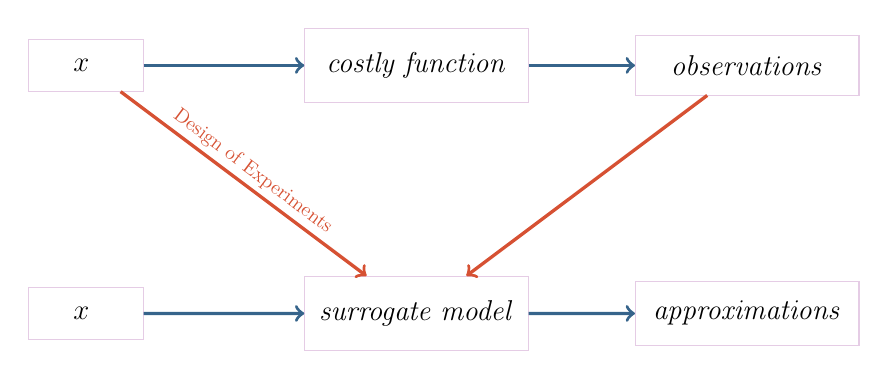
\begin{tikzpicture}[scale=0.7, every node/.style={scale=0.6}]

      % \tikzstyle{Sim}=[rectangle, draw=MonBleu!20, fill=MonBleu!0];
      % \tikzstyle{Meta}=[rectangle, draw=Orange!40, fill=MonBleu!0];
      \tikzstyle{Mes}=[rectangle, draw=violet!20, fill=violet!0];

        \node[Mes](MesIn) at (-6, 0) {
          \parbox{2.2cm}{ %
            \centering
            \LARGE
            \vspace{3mm}
            $x$
            \vspace{3mm}
          }};

        \node[Mes](Mes) at (0, 0) {
          \parbox{4.5cm}{ %
            \centering
            \LARGE
            \vspace{4mm}
            \textit{costly function}\\
            \vspace{4mm}
          }};

        \node[Mes](MesOut) at (6, 0) {
        \parbox{4.5cm}{ %
            \centering
            \LARGE
            \vspace{3mm}
          \textit{observations}\\
            \vspace{3mm}
        }};
        \draw[->, very thick, draw=MonBleu] (MesIn) -- (Mes.west);
        \draw[->, very thick, draw=MonBleu] (Mes) -- (MesOut.west);

        \node[Mes](MetaIn) at (-6, -4.5) {
          \parbox{2.2cm}{ %
          \centering
            \LARGE
            \vspace{3mm}
            $x$
            \vspace{3mm}
          }};

        \node[Mes](Meta) at (0, -4.5) {
          \parbox{4.5cm}{ %
            \centering
            \LARGE
            \vspace{4mm}
            \textit{surrogate model}\\
            \vspace{4mm}
          }};

        \node[Mes](MetaOut) at (6.0, -4.5) {
        \parbox{4.5cm}{ %
            \centering
            \LARGE
            \vspace{3mm}
          \textit{approximations}\\
            \vspace{3mm}
        }};

        \draw[->, very thick, draw=MonBleu] (MetaIn) -- (Meta.west);
        \draw[->, very thick, draw=MonBleu] (Meta) -- (MetaOut.west);

        \draw[->, very thick, draw=Orange!80] (MesIn) -- (Meta)
        node [above, midway, sloped, Orange!80] {\large Design of Experiments};
        \draw[->, very thick, draw=Orange!80] (MesOut)  -- (Meta);
        %node [above, midway, sloped, Orange!80] {\large réponses};

    \end{tikzpicture}
    \end{figure}
In practice, it is risky to take decisions based only on the model...\\
\vspace{3mm}
On the other hand, the model can be used to guide us in the search for the optimum.
\end{frame}

%%%%%%%%%%%%%%%%%%%%%%%%%%%%%%%%%%%%%%%%%%%%%%%%%%%%%%
\begin{frame}{}
\textbf{Global optimization} methods are a trade-off between
\begin{itemize}
	\item Exploitation of past good results
	\item Exploration of the space
\end{itemize}
\vspace{3mm}
\begin{center}
\textbf{How can GPR models be helpful?}\\
\includegraphics[height=5cm]{4_optimization/figures/python/ego_0}
\end{center}
\end{frame}

%%%%%%%%%%%%%%%%%%%%%%%%%%%%%%%%%%%%%%%%%%%%%%%%%%%%%%
\begin{frame}{}
In our example, the best observed value is 1.79
\begin{center}
\includegraphics[height=5cm]{4_optimization/figures/python/ego_improv}
\end{center}
Various criteria can be studied
\begin{itemize}
	\item probability of improvement
	\item Expected improvement
\end{itemize}
\end{frame}

%%%%%%%%%%%%%%%%%%%%%%%%%%%%%%%%%%%%%%%%%%%%%%%%%%%%%%
\begin{frame}{}
\textbf{Probability of Improvement:}
$$PI(x) = cdf \left(\frac{\min(F) - m(x)}{\sqrt{(c(x,x))}} \right)$$
\begin{center}
\includegraphics[height=5cm]{4_optimization/figures/python/ego_PI}
\end{center}
\end{frame}

%%%%%%%%%%%%%%%%%%%%%%%%%%%%%%%%%%%%%%%%%%%%%%%%%%%%%%
\begin{frame}{}
The point with the highest PI is often very close to the best observed value. We can show that there is a $x$ in the neighbourhood of $x^*$ such that $PI(x) \geq 0.5$.\\
\vspace{5mm}
For such points, the improvement cannot be large... \\
\vspace{3mm}
Can we find another criterion?
\end{frame}

%%%%%%%%%%%%%%%%%%%%%%%%%%%%%%%%%%%%%%%%%%%%%%%%%%%%%%
\begin{frame}{}
\textbf{Expected Improvement:}
\begin{equation*}
\begin{split}
E&I(x) =  \int_{-\infty}^{\min(F)} \max\left(0,Y(x)\right) ~dY(x) = \dots = \\
& \sqrt{c(x,x)} (u(x) cdf(u(x)) + pdf(u(x))) \quad \text{ with } u(x) = \frac{\min(F) - m(x)}{\sqrt{(c(x,x))}}
\end{split}
\end{equation*}
%\qquad with $ \displaystyle u(x) = \frac{\min(F) - m(x)}{\sqrt{(c(x,x))}}$
\begin{center}
\includegraphics[height=5cm]{4_optimization/figures/python/ego_EI0}
\end{center}
\end{frame}

%%%%%%%%%%%%%%%%%%%%%%%%%%%%%%%%%%%%%%%%%%%%%%%%%%%%%%
\begin{frame}{Expected Improvement}
Let's see how it works... iteration 1
\begin{center}
\includegraphics[height=5cm]{4_optimization/figures/python/ego_EI1}
\end{center}
\end{frame}

%%%%%%%%%%%%%%%%%%%%%%%%%%%%%%%%%%%%%%%%%%%%%%%%%%%%%%
\begin{frame}[noframenumbering]{Expected Improvement}
Let's see how it works... iteration 2
\begin{center}
\includegraphics[height=5cm]{4_optimization/figures/python/ego_EI2}
\end{center}
\end{frame}

%%%%%%%%%%%%%%%%%%%%%%%%%%%%%%%%%%%%%%%%%%%%%%%%%%%%%%
\begin{frame}[noframenumbering]{Expected Improvement}
Let's see how it works... iteration 3
\begin{center}
\includegraphics[height=5cm]{4_optimization/figures/python/ego_EI3}
\end{center}
\end{frame}

%%%%%%%%%%%%%%%%%%%%%%%%%%%%%%%%%%%%%%%%%%%%%%%%%%%%%%
\begin{frame}[noframenumbering]{Expected Improvement}
Let's see how it works... iteration 4
\begin{center}
\includegraphics[height=5cm]{4_optimization/figures/python/ego_EI4}
\end{center}
\end{frame}

%%%%%%%%%%%%%%%%%%%%%%%%%%%%%%%%%%%%%%%%%%%%%%%%%%%%%%
\begin{frame}[noframenumbering]{Expected Improvement}
Let's see how it works... iteration 5
\begin{center}
\includegraphics[height=5cm]{4_optimization/figures/python/ego_EI9}
\end{center}
\end{frame}

%%%%%%%%%%%%%%%%%%%%%%%%%%%%%%%%%%%%%%%%%%%%%%%%%%%%%%
\begin{frame}{Expected Improvement}
This algorithm is called \textbf{Efficient Global Optimization} (EGO, Jones et al., 1998):
\begin{enumerate}
	\item make an initial design of experiments $X$ and calculate the associated $F$, $t = \mathtt{length}(F)$
	\item built a GP from $(X,F)$ (max. log-likelihood on $\sigma$ and $\theta_i$'s)
	\item $X_{t+1}= \arg \max_x EI(x)$
	\item calculate $F_{t+1}=f(X_{t+1})$, increment $t$
	\item stop ($t>t^\text{max}$) or go to {\color{blue}2.}
\end{enumerate}
\vspace{5mm}
\begin{itemize}
	\item[+] EGO provides a good trade-off between exploitation and exploration without arbitrary parameters.
	\item[+] It requires few function observations (10 in the example) to get close to optimal regions.
\end{itemize}
%\begin{example}
%From the previous 5 iterations, we obtain $1.44e39$ for the conditioning of the covariance matrix. Eigenvalues are
%$$ (67.70,\  24.86,\  5.13,\  1.68,\  0.45,\  0.16,\  0.01,\  0.00,\  0.00,\ 0.00) $$
%\end{example}
\end{frame}

%%%%%%%%%%%%%%%%%%%%%%%%%%%%%%%%%%%%%%%%%%%%%%%%%%%%%%
%\begin{frame}{}
%\begin{exampleblock}{Illustration for $d=6$ (Hartman)}
%	Illustration in higher dimension
%\begin{center}
%\includegraphics[height=5.5cm]{4_optimization/figures/egoHartman} \includegraphics[height=5.5cm]{4_optimization/figures/egoHartman2}
%\end{center}
%\small Source: \textit{DiceOptim}, Roustant, Ginsbourger and Deville, 2009.
%\end{exampleblock}
%\end{frame}

%%%%%%%%%%%%%%%%%%%%%%%%%%%%%%%%%%%%%%%%%%%%%%%%%%%%%%
\begin{frame}{}
\begin{exampleblock}{Example in 5d: surface displacements misfit minimization}
$\Rightarrow$ demo with \texttt{mainInversionPunctualDisplSource.R}\\
!!! normalize the data: WLS has a few very large values, it is always $>0$: make it more gaussian, 
$\mathtt{wls}\_norm = \log(1+\mathtt{wls})$ and all $x$'s and $\mathtt{wls}\_norm$ between 0 and 1.
\begin{minipage}[c]{0.6\textwidth}
\begin{center}
\includegraphics[width=\textwidth]{4_optimization/figures/misfit_learn_set} 
\end{center}
\end{minipage}
\hspace{0.3cm}
\begin{minipage}[c]{0.30\textwidth}
{\small 100 $\{xs,ys,zs,a,p\}$ points chosen through an optimized Latin Hypercube Sampling 
(\texttt{R} libraries \texttt{DiceDesign} or \texttt{lhs}).}\\
\end{minipage}
\end{exampleblock}
\end{frame}

%%%%%%%%%%%%%%%%%%%%%%%%%%%%%%%%%%%%%%%%%%%%%%%%%%%%%%
\begin{frame}{}
\small (demo with \texttt{mainInversionPunctualDisplSource.R}, cont.)
\begin{center}
\includegraphics[width=0.7\textwidth]{4_optimization/figures/misfit_test_set} 
\end{center}
{\tiny 110 random $\{xs,ys,zs,a,p\}$ test points.}\\
\end{frame}

%%%%%%%%%%%%%%%%%%%%%%%%%%%%%%%%%%%%%%%%%%%%%%%%%%%%%%
\begin{frame}{}
\small (demo with \texttt{mainInversionPunctualDisplSource.R}, cont.)
\begin{center}
\includegraphics[width=0.9\textwidth]{4_optimization/figures/misfit_test_set_2} 
\end{center}
{\tiny 110 test points.}\\
\end{frame}

%%%%%%%%%%%%%%%%%%%%%%%%%%%%%%%%%%%%%%%%%%%%%%%%%%%%%%
\begin{frame}{}
\small (demo with \texttt{mainInversionPunctualDisplSource.R}, cont.)\\
\small EGO parameters: anisotropic Mat\`ern 5/2 kernel, GP updated (log-likelihood maximized) every 5 added points, BFGS with bounded variables (from \texttt{optim()} function) restarted from random initial points for maximizing log-likelihood and EI.
\begin{minipage}[c]{0.6\textwidth}
\begin{center}
\includegraphics[width=\textwidth]{4_optimization/figures/misfit_EGO_conv} 
\end{center}
\end{minipage}
\hspace{0.3cm}
\begin{minipage}[c]{0.3\textwidth}
Preferential sampling of good regions of $S$, but global therefore sometimes increasing WLS.
Lower bound on $\theta_i$'s increased from 0.08 to 0.1 at $t=250$ ($x_i$'s and $\theta_i$'s
normed between 0 and 1).
\end{minipage}
\end{frame}

%%%%%%%%%%%%%%%%%%%%%%%%%%%%%%%%%%%%%%%%%%%%%%%%%%%%%%
\begin{frame}{}
\small (demo with \texttt{mainInversionPunctualDisplSource.R}, cont.)
\begin{minipage}[c]{0.6\textwidth}
\begin{center}
\includegraphics[width=\textwidth]{4_optimization/figures/pairs_X_old_new} 
\end{center}
\end{minipage}
\hspace{0.3cm}
\begin{minipage}[c]{0.3\textwidth}
Black: LHS initial points. \\
Blue: EGO points.\\
\vskip\baselineskip
Note the patterns in new points. Accumulation at lower bound of $a$ and mid interval of $p$ before $t=250$.
\end{minipage}
\end{frame}

%%%%%%%%%%%%%%%%%%%%%%%%%%%%%%%%%%%%%%%%%%%%%%%%%%%%%%
\begin{frame}{}
\small (demo with \texttt{mainInversionPunctualDisplSource.R}, cont.)
\begin{minipage}[c]{0.6\textwidth}
\begin{center}
\includegraphics[width=\textwidth]{4_optimization/figures/pairs_X_good_15percent} 
\end{center}
\end{minipage}
\hspace{0.3cm}
\begin{minipage}[c]{0.3\textwidth}
15\% best sampled points. Note the ``function'' for the $(a,p)$ pair, i.e., $a^\star(p^\star)$.
\end{minipage}
\end{frame}

%%%%%%%%%%%%%%%%%%%%%%%%%%%%%%%%%%%%%%%%%%%%%%%%%%%%%%
\begin{frame}{}
\small (demo with \texttt{mainInversionPunctualDisplSource.R}, cont.)
\mbox{ % mbox to avoid linebreak
\begin{minipage}[c]{0.56\textwidth}
\begin{center}
\includegraphics[width=\textwidth]{4_optimization/figures/non_identif_a_p} 
\end{center}
\end{minipage}
\hspace{0.3cm}
\begin{minipage}[c]{0.4\textwidth}
Mogi model only dependency in $a$ and $p$ is through $a^3 \times p$: it is not identifiable. \\
\vskip\baselineskip
EGO tells it by preferential sampling in the valley 
$$a^3 \times p = \text{const.} = {a^\star}^3 \times p^\star$$
\end{minipage}
} % end mbox
Other EGO output: a statistical model of WLS. \\
The last length scales are an indication of the 
sensitivity of WLS to each variable: $a$, $p$ and $zs$ are very sensitive 
($\theta_i$'s small, in $[0.08,0.1]$), $xs$ a little sensitive ($\theta \text{ in } [0.1,2.5]$) 
and $ys$ insensitive ($\theta \approx 3$).
\end{frame}

%%%%%%%%%%%%%%%%%%%%%%%%%%%%%%%%%%%%%%%%%%%%%%%%%%%%%%
\begin{frame}{}
\begin{exampleblock}{Difficulties and challenges with EGO}
\begin{itemize}
\item Standard GPs are limited to $n \approx 1000$ points (covariance matrix inversion).
\item EGO clusters points in good regions, the covariance matrix may become ill-conditionned 
if length scales $\theta_i$ are too small.
\item Although the method perfectly applies to large dimensional spaces ($d>100$), larger $d$ 
may require larger $n$, back 2 lines above.
\item EGO does not converge in the traditional sense: it creates dense samples in the volume of $S$. 
The efficiency comes from the order in which points are sampled.
\end{itemize}
$\Rightarrow$ these are the topics of current research. Let's mention a few extensions next.
\end{exampleblock}
\end{frame}

%%%%%%%%%%%%%%%%%%%%%%%%%%%%%%%%%%%%%%%%%%%%%%%%%%%%%%
\begin{frame}{}
One way to improve the conditioning of the covariance matrix is to replace two values that are close-by by one function value and one derivative:
\begin{center}
  \begin{tabular}{ccc}
\includegraphics[height=4cm]{4_optimization/figures/python/osborn0} &
\includegraphics[height=4cm]{4_optimization/figures/Rightarrow} &
\includegraphics[height=4cm]{4_optimization/figures/python/osborn1} \\
Cond. = 3842 & & Cond. = 10
  \end{tabular}
\end{center}
This can be generalised to higher orders \alert{$\rightarrow$} Taylor expansion\\
\small see articles from M. Osborn
\end{frame}

%%%%%%%%%%%%%%%%%%%%%%%%%%%%%%%%%%%%%%%%%%%%%%%%%%%%%%
\begin{frame}{}
If we know the computational budget in advance, adding new points at the \textbf{best one step ahead location} is not optimal.\\
\vspace{5mm}
Some improvements have been made toward this
\begin{itemize}
	\item Batch EGO
	\item Parallelization of the algorithm
\end{itemize}
\vspace{5mm}
\small see works from D. Ginsbourger
\end{frame}

%%%%%%%%%%%%%%%%%%%%%%%%%%%%%%%%%%%%%%%%%%%%%%%%%%%%%%
%%%%%%%%%%%%%%%%%%%%%%%%%%%%%%%%%%%%%%%%%%%%%%%%%%%%%%
\section[Robust optim.]{Robust optimization}
\subsection{}

%%%%%%%%%%%%%%%%%%%%%%%%%%%%%%%%%%%%%%%%%%%%%%%%%%%%%%
\begin{frame}{}
Robust optimization may mean various things:
\begin{itemize}
	\item There is observation noise on the output
	\item Some input variables are uncertain
	\item Model is uncertain
\end{itemize}
\vspace{2mm}
\begin{example}
\begin{columns}[c]
\column{3cm}
	\includegraphics[height=4cm]{4_optimization/figures/RLRrobust}
\column{5cm}
	a +/- 1mm dispersion in the manufacturing of a car cylinder head  can degrade its performance (g CO2/km) by -20\% (worst case)\\
\end{columns}
\vspace{3mm}
	\small Source: Talk from R. Le Riche at the Porquerolles Summer School, 2014
\end{example}
\end{frame}

%%%%%%%%%%%%%%%%%%%%%%%%%%%%%%%%%%%%%%%%%%%%%%%%%%%%%%
\begin{frame}{}
% \begin{example}
% Here is a basic example:
% \begin{center}
% \includegraphics[height=5cm]{4_optimization/figures/optim_rob_a}\\
% Which input is the best?
% \end{center}
% \end{example}
% \end{frame}

% %%%%%%%%%%%%%%%%%%%%%%%%%%%%%%%%%%%%%%%%%%%%%%%%%%%%%%
% \begin{frame}[noframenumbering]{}
\begin{example}
Here is a basic example:
\begin{center}
\includegraphics[height=5cm]{4_optimization/figures/optim_rob_b}\\
Which input is the best?
\end{center}
\end{example}
\end{frame}

%%%%%%%%%%%%%%%%%%%%%%%%%%%%%%%%%%%%%%%%%%%%%%%%%%%%%%
\begin{frame}[noframenumbering]{}
\begin{example}
A non Gaussian example
\begin{center}
\includegraphics[height=5cm]{4_optimization/figures/optim_rob_c}\\
In some cases, we may want to optimize the worst case scenario.
\end{center}
\end{example}
\end{frame}

%%%%%%%%%%%%%%%%%%%%%%%%%%%%%%%%%%%%%%%%%%%%%%%%%%%%%%
\begin{frame}{}
Can EGO be adapted when observations are noisy?\\
\vspace{5mm}
First of all, using the current best observation as a minimum does not make much sense...\\
\vspace{5mm}
Some solutions are
\begin{itemize}
	\item[S1] Build a new model that interpolates $m(X)$ at $X$.
	\item[S2] Include observation noise and replace $\min(F)$ by $\min(m(X))$ in the EI expression
	\item[S3] Similar to 2 but consider an Expected Mean Improvement.
\end{itemize}
\end{frame}

%%%%%%%%%%%%%%%%%%%%%%%%%%%%%%%%%%%%%%%%%%%%%%%%%%%%%%
\begin{frame}{Solution 1}
iteration 0
\begin{center}
\includegraphics[height=5cm]{4_optimization/figures/python/ego_EI1n0}
\end{center}
\end{frame}

%%%%%%%%%%%%%%%%%%%%%%%%%%%%%%%%%%%%%%%%%%%%%%%%%%%%%%
\begin{frame}[noframenumbering]{Solution 1}
iteration 1
\begin{center}
\includegraphics[height=5cm]{4_optimization/figures/python/ego_EI1n1}
\end{center}
\end{frame}

%%%%%%%%%%%%%%%%%%%%%%%%%%%%%%%%%%%%%%%%%%%%%%%%%%%%%%
\begin{frame}[noframenumbering]{Solution 1}
iteration 2
\begin{center}
\includegraphics[height=5cm]{4_optimization/figures/python/ego_EI1n2}
\end{center}
\end{frame}

%%%%%%%%%%%%%%%%%%%%%%%%%%%%%%%%%%%%%%%%%%%%%%%%%%%%%%
\begin{frame}[noframenumbering]{Solution 1}
iteration 3
\begin{center}
\includegraphics[height=5cm]{4_optimization/figures/python/ego_EI1n3}
\end{center}
\end{frame}

%%%%%%%%%%%%%%%%%%%%%%%%%%%%%%%%%%%%%%%%%%%%%%%%%%%%%%
\begin{frame}[noframenumbering]{Solution 1}
iteration 4
\begin{center}
\includegraphics[height=5cm]{4_optimization/figures/python/ego_EI1n4}
\end{center}
\end{frame}

%%%%%%%%%%%%%%%%%%%%%%%%%%%%%%%%%%%%%%%%%%%%%%%%%%%%%%
%%%%%%%%%%%%%%%%%%%%%%%%%%%%%%%%%%%%%%%%%%%%%%%%%%%%%%
\section[Related problems]{Related problems}
\subsection{}

%%%%%%%%%%%%%%%%%%%%%%%%%%%%%%%%%%%%%%%%%%%%%%%%%%%%%%
\begin{frame}{}
Some related optimization problems are:
\begin{itemize}
	\item calibration problems
	\item probability computations
\end{itemize}
\vspace{8mm}
Some algorithms with an EGO spirit can be applied:
\begin{itemize}
 	\item SUR methods
 \end{itemize}
\end{frame}

%%%%%%%%%%%%%%%%%%%%%%%%%%%%%%%%%%%%%%%%%%%%%%%%%%%%%%
\begin{frame}{}
We want to find the input(s) such that f(x) = 3.2
\begin{center}
\includegraphics[height=5cm]{4_optimization/figures/python/inv}
\end{center}
\end{frame}

%%%%%%%%%%%%%%%%%%%%%%%%%%%%%%%%%%%%%%%%%%%%%%%%%%%%%%
\begin{frame}[noframenumbering]{}
iteration 0:
\begin{center}
\includegraphics[height=5cm]{4_optimization/figures/python/invproba}
\end{center}
\end{frame}

%%%%%%%%%%%%%%%%%%%%%%%%%%%%%%%%%%%%%%%%%%%%%%%%%%%%%%
\begin{frame}[noframenumbering]{}
iteration 1:
\begin{center}
\includegraphics[height=5cm]{4_optimization/figures/python/invproba1}
\end{center}
\end{frame}

%%%%%%%%%%%%%%%%%%%%%%%%%%%%%%%%%%%%%%%%%%%%%%%%%%%%%%
\begin{frame}[noframenumbering]{}
iteration 2:
\begin{center}
\includegraphics[height=5cm]{4_optimization/figures/python/invproba2}
\end{center}
\end{frame}

%%%%%%%%%%%%%%%%%%%%%%%%%%%%%%%%%%%%%%%%%%%%%%%%%%%%%%
\begin{frame}[noframenumbering]{}
iteration 3:
\begin{center}
\includegraphics[height=5cm]{4_optimization/figures/python/invproba3}
\end{center}
\end{frame}


%%%%%%%%%%%%%%%%%%%%%%%%%%%%%%%%%%%%%%%%%%%%%%%%%%%%%%
%%%%%%%%%%%%%%%%%%%%%%%%%%%%%%%%%%%%%%%%%%%%%%%%%%%%%%
\section[Conclusions]{Concluding remarks}
\subsection{}
%%%%%%%%%%%%%%%%%%%%%%%%%%%%%%%%%%%%%%%%%%%%%%%%%%%%%%
\begin{frame}{}
\begin{exampleblock}{Conclusions}
\begin{itemize}
\item Gaussian Processes offer a versatile framework for building statistical models of physical models.
\item Main assumptions: the phenomenon is Gaussian, functional choice of covariance function (kernel).
\item Knowledge transfer from the physical to the statistical model: through data + expertise guiding 
the choice of kernel.
\item Complementary to the physical model, useful for decision making.
\end{itemize}
\end{exampleblock}

\end{frame}



\end{document}
